\documentclass[a4paper,10pt]{report}
\usepackage{Cours}
\usepackage{delarray}
\usepackage{fancybox}
\newcommand{\Sum}[2]{\ensuremath{\textstyle{\sum\limits_{#1}^{#2}}}}
\newcommand{\Int}[2]{\ensuremath{\mathchoice%
	{{\displaystyle\int_{#1}^{#2}}}
	{{\displaystyle\int_{#1}^{#2}}}
	{\int_{#1}^{#2}}
	{\int_{#1}^{#2}}
	}}
\usepackage{pstricks-add}



\begin{document}
% \everymath{\displaystyle}

\maketitle{Chapitre 9}{Intégrales généralisées}

\noindent Dans la suite $\mathbb{K}= \mathbb{R}$ ou $\mathbb{C}$. Si rien n'est précisé, une fonction définie sur un intervalle est à valeurs complexes.

\section{Intégrale sur un segment de fonctions continues par morceaux}

\subsection{Fonctions continues par morceaux}

\begin{defin}
Soient $(a,b) \in \mathbb{R}^2$ tel que $a \leq b$ et $f$ une fonction définie sur $[a,b]$.\\
La fonction $f$ est dite \textit{continue par morceaux} sur le segment $[a,b]$ si il existe une subdivision \linebreak $a_0 = a < a_1 < a_2 < \dots < a_n =b$ telle que les restrictions de $f$ sur chaque intervalle ouvert $]a_i,a_{i+1}[$ (où $i \in \Interv0{n-1}$) admettent un prolongement continu à l'intervalle fermé $[a_i,a_{i+1}]$.
\end{defin}

\begin{rem} La subdivision $(a_0, \ldots, a_n)$ est dite adaptée à $f$. Elle n'est pas unique.
\end{rem}

\medskip

%
%\pagebreak
%
\begin{center}
\textit{Exemple d'une courbe d'une fonction continue par morceaux à valeurs réelles}
\end{center}

\begin{center}
 \begin{tikzpicture}[>=stealth,scale=1]
\draw[->,color=black] (-0.6,0) -- (6.6,0) node[below] {$x$};
\foreach \x in {1,2,...,6}
\draw[shift={(\x,0)},color=black] (0pt,2pt) -- (0pt,-2pt) node[below] {\footnotesize $\x$};
\draw[->,color=black] (0,-0.6) -- (0,4.6) ;
\foreach \y in {1,2,...,4}
\draw[shift={(0,\y)},color=black] (2pt,0pt) -- (-2pt,0pt) node[left] {\footnotesize $\y$};
\draw[color=black] (0pt,-10pt) node[left] {\footnotesize $0$};
\clip(-0.6,-0.6) rectangle (6.6,4.6);
\draw[smooth,samples=100,domain=0:2] (0,3) node {$\bullet$} plot(\x,{sin(180*\x)+3-\x}) node {$\circ$};
\draw (2,0) node {$\circ$} (2,4) node {$\bullet$} (6,3) node {$\bullet$};
\draw[smooth,samples=100,domain=2:5] plot(\x,{\x-1-((\x-3.5)/1.5)^2}) node {$\bullet$};
\draw[o-o] (5,2)--(6,2);
\end{tikzpicture}
\end{center}

\medskip
 
\begin{center}
\textit{Exemple d'une courbe d'une fonction non continue par morceaux à valeurs réelles}
\end{center}
% 
%\begin{cex} La fonction $h$ définie sur $[0,6]$ et dont la courbe est 
 \begin{center}
  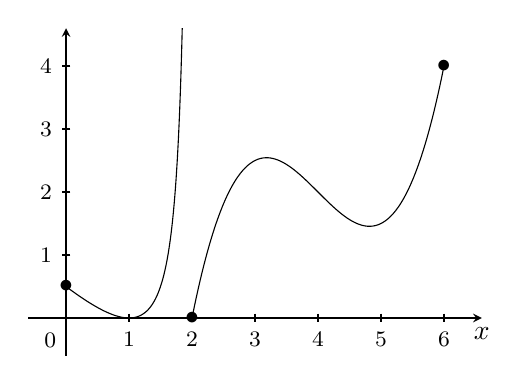
\begin{tikzpicture}[>=stealth,scale=0.8]
\draw[->,color=black] (-0.6,0) -- (6.6,0) node[below] {$x$};
\foreach \x in {1,2,...,6}
\draw[shift={(\x,0)},color=black] (0pt,2pt) -- (0pt,-2pt) node[below] {\footnotesize $\x$};
\draw[->,color=black] (0,-0.6) -- (0,4.6);
\foreach \y in {1,2,...,4}
\draw[shift={(0,\y)},color=black] (2pt,0pt) -- (-2pt,0pt) node[left] {\footnotesize $\y$};
\draw[color=black] (0pt,-10pt) node[left] {\footnotesize $0$};
\clip(-0.6,-0.6) rectangle (6.6,4.6);
\draw[smooth,samples=100,domain=0:1.9] plot(\x,{1/(2-\x)-\x});
\draw (0,0.5) node {$\bullet$};
\draw (2,0) node {$\bullet$};
\draw[smooth,samples=100,domain=2:6] plot(\x,{0.5*(\x-4)^3-(\x-6)}) node {$\bullet$};
\end{tikzpicture}
\end{center}

%\end{cex}
%
%\begin{exems} 
%\item la fonction $f$ définie sur $[0,5]$ par $f(x) = \begin{cases} x+1 &\text{si } x \leq 2 \\ \ln x & \text{si } x > 2 \end{cases}$ est continue par morceaux sur $[0,5]$.
%\item La fonction $f$ définie sur $[-1,1]$ par $f(x) = \begin{cases} 1 &\text{si } x \leq 0 \\ \dfrac{1}{x} & \text{si } x >0 \end{cases}$ n'est pas continue par morceaux sur $[-1,1]$.
%\end{exems}

\begin{defin} Une fonction $f$ est \textit{continue par morceaux} sur un intervalle $I$ si elle est continue par morceaux sur tout segment $[a,b]$ inclus dans $I$.
\end{defin}

\begin{rem} La définition est cohérente dans le cas où $I$ est un segment car dans ce cas, $f$ est bien continue par morceaux sur tout sous-segment.
\end{rem}

\begin{prop} L'ensemble des fonctions continues par morceaux sur $I$ à valeurs dans $\mathbb{K}$, notée $\mathcal{CM}(I,\mathbb{K})$ est un sous-espace vectoriel de l'ensemble des fonctions de $I$ à valeurs dans $\mathbb{K}$.
\end{prop}

\begin{preuve} On utilise la méthode des trois points :

\begin{itemize}
\item $\mathcal{CM}(I,\mathbb{K}) \subset \mathcal{F}(I, \mathbb{K})$.
\item L'application nulle est continue par morceaux sur $I$.
\item Soient $f$, $g$ deux fonctions continues par morceaux sur $I$ et $\alpha \in \mathbb{K}$. Fixons un segment $[a,b]$ de $I$. Remarquons d'abord que toute subdivision adaptée à $f$ sur $[a,b]$ est aussi adaptée à $\alpha f$. Donnons nous deux subdivisions $(a_0, a_1, \ldots, a_n)$ et $(b_0,b_1, \ldots, b_p)$ de $f$ et $g$ sur $[a,b]$(avec $n,p \in \mathbb{N}^*$). On crée alors l'union de ces deux subdivisions (en rangeant dans l'ordre croissant ces $n+p$ nombres et en enlevant les répétitions). Cette nouvelle subdivision est alors une subdivision adaptée à $\alpha f + g$ sur $[a,b]$. Pour cela il suffit de remarquer que si $c$ est un point de la nouvelle subdivision alors soit $c$ est un point des deux subdivisions précédentes et il n'y a rien à vérifier et si $c$ est un point de la subdivision de l'une des deux uniquement alors $c$ est un point où l'autre est continue. Ainsi $\alpha f+g$ est continue par morceaux sur tout segment de $I$ donc sur $I$.
\end{itemize}
\end{preuve}

\begin{prop} Toute fonction continue par morceaux sur un segment $[a,b]$ est bornée sur ce segment.
\end{prop}



\subsection{Intégrale sur un segment d'une fonction continue par morceaux}

\begin{defip} 
Soient $(a,b) \in \mathbb{R}^2$ tel que $a \leq b$ et $f$ une fonction continue par morceaux sur $[a,b]$.\\
Soit $a_0 = a < a_1 < a_2 < \dots < a_n =b$ une subdivision adaptée à $f$. Pour tout $i \in \Interv{0}{n-1}$, on note $\tilde{f}_i$ le prolongement continu de $f$ sur $[a_i,a_{i+1}]$. On définit l'intégrale de $f$ sur $[a,b]$ par :
$$ \int_{a}^b f(t) \dt = \int_{a_0}^{a_1} \tilde{f}_0(t) \dt + \int_{a_1}^{a_2} \tilde{f}_1(t) \dt + \cdots + \int_{a_{n-1}}^{a_n} \tilde{f}_{n-1}(t) \dt$$
Cette définition ne dépend pas de la subdivision choisie.
\end{defip}

\begin{preuve} Donnons juste l'idée : si l'on considère une subdivision adaptée à $f$ sur $[a,b]$, on obtient une autre subdivision adapté à $f$ en \og enlevant \fg les points de la première subdivision où $f$ est continue (qui, en un sens, sont inutiles). En faisant cela, on se ramène à une subdivision \og minimale \fg et on peut alors vérifier que la définition ne dépend pas de la subdivision choisie.
\end{preuve}

\subsection{Propriétés}

\noindent Les propriétés des intégrales des fonctions continues sur un segment se généralisent, pour la plupart, aux intégrales des fonctions continues par morceaux. Nous ne donnons pas les preuves de celles-ci. Dans toute la suite, $(a,b)$ est un couple de réels tels que $a \leq b$.

\begin{prop}[Linéarité] Soient $f,g$ deux fonctions continues par morceaux sur $[a,b]$ et à valeurs dans $\mathbb{K}$ et $\lambda \in \mathbb{K}$. Alors :
$$ \int_{a}^b (\lambda f(t) + g(t)) \dt = \lambda \int_{a}^b  f(t) \dt +  \int_{a}^b  g(t) \dt$$
\end{prop}

\begin{prop}[Relation de Chasles] Soient $f$ une fonction continue par morceaux sur $[a,b]$ et à valeurs dans $\mathbb{K}$ et $c \in [a,b]$. Alors :
$$ \int_{a}^b f(t) \dt = \int_{a}^c f(t) \dt + \int_{c}^b f(t) \dt $$
\end{prop}

\begin{prop}[Positivité] Soient $f$ une fonction continue par morceaux sur $[a,b]$ et à valeurs réelles \textit{positives}. Alors $\Int{a}{b} f(t) \dt \geq 0$.
\end{prop}

\begin{prop}[Croissance] Soient $f,g$ deux fonctions continues par morceaux sur $[a,b]$ à valeurs réelles. Si pour tout $t \in [a,b]$, $f(t) \leq g(t)$ alors :
$$\int_{a}^{b} f(t) \dt  \leq \int_{a}^{b} g(t) \dt $$
\end{prop}

\begin{prop}[Stricte positivité]  Soit $f$ une fonction continue sur $[a,b]$ et à valeurs réelles \textit{positives}. 

\begin{itemize}
\item Si il existe $x_0 \in [a,b]$ tel que $f(x_0)>0$ alors $\Int{a}{b} f(t) \dt>0$.
\item Si $\Int{a}{b} f(t) \dt =0$ alors $f$ est la fonction nulle sur $[a,b]$.
\end{itemize}
\end{prop}

\begin{att} Cette proposition est fausse en toute généralité si la fonction est continue par morceaux : il suffit de penser à la fonction $f$ définie sur $[0,1]$ par $f(x)=0$ si $x \neq \frac{1}{2}$ et par $f(\frac{1}{2})=1$.
\end{att}

\begin{prop} Soit $f$ une fonction continue par morcreaux sur $[a,b]$ à valeurs dans $\mathbb{K}$. Alors $\vert f \vert$ est continue par morceaux   sur $[a,b]$ et à valeurs positives et :
$$ \left\vert \int_{a}^b f(t) \dt \right\vert \leq \int_{a}^b \vert f(t) \vert \dt $$
\end{prop}

\begin{prop} Soient $f$, $g$ deux fonctions continues par morceaux sur $[a,b]$ et à valeurs dans $\mathbb{K}$. Si $f$ et $g$ coïncident sauf en un nombre fini de points alors :
$$ \int_{a}^b f(t) \dt = \int_{a}^b g(t) \dt $$
\end{prop}

\subsection{Quelques méthodes de calcul}
\subsubsection{Méthodes du chapitre 8}

\begin{itemize}
\item En déterminant une primitive.
\item Par linéarisation.
\item Par intégration par parties.
\item Par changement de variable.
\item En utilisant une fonction complexe.
\end{itemize}

\medskip

\noindent Il est très important de retravailler sérieusement les exercices du chapitre 8. 

\subsubsection{Changement de variable}

\begin{prop} Soient $I$ et $J$ deux intervalles de $\mathbb{R}$, $f$ une fonction continue par morceaux sur $I$ et $\varphi : J \rightarrow I$ une fonction de classe $\mathcal{C}^1$ et strictement monotone. Pour tout $(\alpha, \beta) \in J^2$, on a :
$$ \int_{\varphi(\alpha)}^{\varphi(\beta)} f(t) \dt = \int_{\alpha}^{\beta} f( \varphi(x)) \varphi'(x) \dx$$
\end{prop}

\newpage

\begin{rem} Dans le cas où $f$ est continue sur $I$, l'hypothèse de stricte monotonie n'est pas utile et on retrouve la formule utilisée en Sup.
\end{rem}

\begin{ex} Calculons $I= \dis \int_{0}^1 \dfrac{1}{ch(t)} \dt$.

\vspace{7cm}
\end{ex}

\begin{ex} Calculons $I= \dis \int_{0}^1 \sqrt{1-t^2} \dt$.

\vspace{7cm}
\end{ex}


\subsubsection{Fractions rationnelles}

\noindent On appelle \textit{fraction rationnelle} tout élément de la forme $\dfrac{A(X)}{B(X)}$ où $(A,B) \in \mathbb{R}[X]^2$ avec $B$ non nul. Pour calculer l'intégrale d'une fonction associée à une fraction rationnelle, on procède de la manière suivante : 

\bigskip

\noindent $\rhd$ On effectue la division euclidienne de $A$ par $B$ : il existe un unique couple $(Q,R) \in \mathbb{R}[X]^2$ tel que :
$$ A(X) = Q(X)B(X) + R(X)$$
avec $\textrm{deg}(R)< \textrm{deg}(B)$. On a ainsi :
$$ \dfrac{A(X)}{B(X)} = Q(X) + \dfrac{R(X)}{B(X)}$$
$Q$ est un polynôme, il suffit donc de savoir calculer l'intégrale de la fonction associée à $\dfrac{R(X)}{B(X)} \cdot$

\medskip

\noindent $\rhd$ On utilise le résultat suivant :

\begin{thm} Si la décomposition de $B$ en produit de facteurs irréductibles de $\mathbb{R}[X]$ est :
$$ B(X) = \lambda \prod_{k=1}^n (X-a_k)^{\alpha_k} \times \prod_{k=1}^m (X^2+ c_k X + d_k)^{\beta_k} $$
Alors il existe une unique décomposition de $\dfrac{R(X)}{B(X)}$ sous la forme :
$$ \sum_{k=1}^n \sum_{i=1}^{\alpha_k} \frac{\alpha_{k,i}}{(X-a_k)^{i}} + \sum_{k=1}^m \sum_{i=1}^{\beta_k} \dfrac{\mu_{k,i} X + \nu_{k,i}}{(X^2+ c_k X + d_k)^i} $$
où les $\alpha_{k,i}$, $\mu_{k,i}$ et $\nu_{k,i}$ sont des réels.
\end{thm}

\begin{ex} Il existe des réels $a,b,c$ et $d$ tels que :
$$ \dfrac{1}{(X-1)^2 (X^2+1)} = \frac{a}{(X-1)} + \frac{b}{(X-1)^2} + \frac{cX+d}{X^2+1}$$
Déterminons ces réels.

\vspace{11cm}
\end{ex}

\medskip 

\noindent $\rhd$ Il reste à savoir déterminer des primitives de fonctions dont l'expression est de la forme :
$$ \frac{1}{(X-a)^m} \quad \hbox{ ou }  \quad\frac{ax+b}{(x^2+px+q)^m} \hbox{ avec } p^2-4q<0$$

\medskip


\noindent \textbf{1.} Une primitive de $x \mapsto \dfrac{1}{(x-a)}$ sur $]-\infty,a[$ ou $]a, + \infty[$ est $x \mapsto \ln( \vert x-a \vert)$.

\medskip

\noindent \textbf{2.} Si $n$ est un entier naturel supérieur ou égal à $2$, une primitive de 
$$x \mapsto \dfrac{1}{(x-a)^n}= (x-a)^{-n}$$ sur $]-\infty,a[$ ou $]a, + \infty[$ est 
$$x \mapsto \dfrac{(x-a)^{-n+1}}{-n+1} = \dfrac{1}{(1-n)(x-a)^{1-n}} $$

\medskip

\noindent \textbf{3.} Pour déterminer une primitive d'une fonction dont l'expression est $\dfrac{1}{x^2+px+q}$ où $p^2-4q<0$, on écrit sous forme canonique le dénominateur et on sa ramène à une expression de la forme :
$$ \hbox{constante} \times \frac{1}{(\ldots)^2+1}$$
ce qui permet de déterminer une primitive à l'aide de la fonction $\arctan$. 

\medskip

\begin{ex} Pour tout $x \in \mathbb{R}$,

\medskip
\medskip

\quad \qquad $\dis \frac{1}{x^2+x+1} =$
 
 \vspace{10cm}
% 
% 
% 
% \frac{1}{\left( x + \frac{1}{2}\right)^2- \frac{1}{4}+1}  \\
% & = \frac{1}{\left( x + \frac{1}{2}\right)^2 + \frac{3}{4}} \\
% &  = \frac{4}{3} \frac{1}{\left(\frac{2}{\sqrt{3}}\left( x + \frac{1}{2}\right)\right)^2 +1} \\
%   &  = \frac{4}{3} \frac{1}{\left(\frac{2x+1}{\sqrt{3}} \right)^2 +1} \\
%    & = \frac{4}{3} \times \frac{\sqrt{3}}{2} \times  \frac{\frac{2}{\sqrt{3}}}{\left(\frac{2x+1}{\sqrt{3}} \right)^2 +1} \\
%  & =\frac{2}{\sqrt{3}}  \times  \frac{\frac{2}{\sqrt{3}}}{\left(\frac{2x+1}{\sqrt{3}} \right)^2 +1} 
%\end{align*}
\noindent Une primitive est ainsi donnée par $\dis x \mapsto \phantom{\frac{2}{\sqrt{3}} \arctan \left( \frac{2x+1}{\sqrt{3}} \right)\cdot}$
\end{ex}

\begin{exa} Déterminer une primitive sur $\mathbb{R}$ de :
$$ x \mapsto \frac{1}{x^2+5x+7}$$
\end{exa}


\noindent \textbf{4.} Pour déterminer une primitive d'une fonction dont l'expression est $\dfrac{ax+b}{x^2+px+q}$, on fait apparaitre la dérivée du dénominateur au numérateur (on détermine une primitive à l'aide de la fonction logarithme népérien), le terme restant se traitant comme au cas précédent.

\medskip

\begin{ex} Pour tout $x \in \mathbb{R}$,
$$ \frac{3x-1}{x^2+x+1} = \; \phantom{\frac{3}{2}} \times \frac{2x+1}{x^2+x+1} - \phantom{\frac{5}{2} \times \frac{1}{x^2+x+1}}$$
Une primitive est ainsi donnée par :

\vspace{3cm}
%\begin{align*}
% x & \mapsto  \dfrac{3}{2} \ln(\vert x^2+x+1 \vert) - \frac{5}{2} \times  \frac{2}{\sqrt{3}} \arctan \left( \frac{2x+1}{\sqrt{3}} \right)\\
%& =  \dfrac{3}{2} \ln( x^2+x+1 ) -  \frac{5}{\sqrt{3}} \arctan \left( \frac{2x+1}{\sqrt{3}} \right)
%\end{align*}
\end{ex}

\begin{exa} Déterminer une primitive sur $\mathbb{R}$ de :
$$ x \mapsto \frac{x+3}{x^2+5x+7}$$
\end{exa}

\noindent \textbf{5.} Pour déterminer une primitive d'une fonction dont l'expression est $\dfrac{ax+b}{(x^2+px+q)^n}$ avec $n$ un entier naturel supérieur ou égal à $2$, on on fait apparaitre la dérivée du dénominateur au numérateur (on détermine une primitive à l'aide de la forme $u'u^{-n}$), le terme restant se ramenant avec un changement de variable à déterminer la primitive suivante :
$$ \int \frac{1}{(1+x^2)^n} \dx$$
Celle-ci se déterminant par intégration par parties successives en partant de $\dis \Int{}{} \dfrac{1}{1+x^2} \dx$

\begin{ex} Déterminons $\Int{a}{b} \dfrac{1}{(x^2+1)^2} \dx$.
%
%\noindent Les fonctions $x \mapsto x$ et $x \mapsto  \dfrac{1}{1+x^2}$ sont de classe $\mathcal{C}^1$ sur $[a,b]$ et de dérivées respectives $x \mapsto 1$ et $x \mapsto \frac{-2x}{(1+x^2)^2}$, on a donc par intégration par parties :
%\begin{align*}
%\dis \int_{a}^b \dfrac{1}{1+x^2} \dx & = \left[ \frac{x}{1+x^2} \right]_a^b - \int_{a}^b x \left( \frac{-2x}{(1+x^2)^2} \right) \dx \\
%& = \left[ \frac{x}{1+x^2} \right]_a^b +2 \int_{a}^b \frac{x^2}{(1+x^2)^2} \dx \\
%& = \left[ \frac{x}{1+x^2} \right]_a^b + 2 \int_{a}^b \frac{1}{1+x^2} \dx - \frac{1}{(1+x^2)^2} \dx \\
%\end{align*}
%Finalement, en isolant l'intégrale cherchée, on obtient :
%$$ \int_{a}^b \frac{1}{(1+x^2)^2} \dx = \frac{1}{2} \int_{a}^b \frac{1}{1+x^2} + \frac{1}{2}\left[ \frac{x}{1+x^2} \right]_a^b $$

\vspace{7cm}

\end{ex}
\begin{ex} Déterminons $\dis \Int{0}{1} \dfrac{3x-1}{(x^2+x+1)^2} \dx$.
%
%\noindent Pour tout $x \in [0,1]$,
%$$ \frac{3x-1}{(x^2+x+1)^2} = \frac{3}{2} \times \frac{2x+1}{(x^2+x+1)^2} - \frac{5}{2} \times \frac{1}{(x^2+x+1)^2} $$
%Une primitive de $x \mapsto \dfrac{2x+1}{(x^2+x+1)^2}= (2x+1)(x^2+x+1)^{-2}$ est donnée par :
%$$ x \mapsto \frac{(x^2+x+1)^{-1}}{-1} = - \frac{1}{x^2+x+1}$$
%On sait de plus que pour tout $x \in [0,1]$,
%$$  \frac{1}{(x^2+x+1)^2} = \frac{1}{\left(\left( x + \frac{1}{2}\right)^2 + \frac{3}{4}\right)^2} = \frac{16}{9}  \frac{1}{\left(\left(\frac{2}{\sqrt{3}}\left( x + \frac{1}{2}\right)\right)^2 + 1 \right)^2}$$
%Ainsi par changement de variable affine $u= \dfrac{2}{\sqrt{3}}\left( x + \frac{1}{2}\right)$, on a :
%$$ \int_{0}^1  \frac{1}{(x^2+x+1)^2} \dx = \frac{16}{9} \frac{\sqrt{3}}{2} \int_{\frac{1}{\sqrt{3}}}^{\sqrt{3}} \frac{1}{(u^2+1)^2} \textrm{d}u$$
%Cette dernière intégrale se calcule à l'aide de l'exemple précédent.

\vspace{10cm}
\end{ex}

%\begin{exa} Exprimer en fonction de $\arctan$ la valeur de :
%$$ I =  \int_{0}^{1} \frac{x}{(x^2+5x+7)^2} \dx$$
%\end{exa}

\section{Intégrales généralisées sur un intervalle quelconque}
\subsection{Intégrales généralisées sur $[a, + \infty[$}

\begin{defin}
Soit $f$ une fonction continue par morceaux sur $[a,\pinf[$ à valeurs réelles ou complexes.
\begin{itemize}
\item On dit que l'intégrale $\int_a^\pinf f(t)\dt$ \textit{converge} lorsque la fonction $x \mapsto \int_a^x f(t) \dt$ admet une limite finie lorsque $x$ tend vers $\pinf$. Dans ce cas, on pose :
\[ \dis \int_a^\pinf f(t) \dt = \phantom{\lim_{x\to \pinf} \int_a^x f(t)\dt} \]
\item Dans le cas contraire, on dit que $\int_a^\pinf f(t)\dt$ \textit{diverge}.
\end{itemize}
\end{defin}

\noindent Une intégrale de la forme précédente est dite \textit{impropre} (ou \textit{généralisée}) en $+ \infty$.

\medskip

\begin{rem} 
Pour tout $x \in [a, + \infty[$, l'intégrale $\int_{a}^x f(t) dt$ existe bien car $f$ est continue par morceaux sur $[a,x]$. On peut donc bien étudier la limite de cette expression quand $x$ tend vers $+\infty$.
\end{rem}

\medskip

\begin{ex}
Étudions la convergence de l'intégrale suivante : $I = \dis \int_{0}^{+ \infty} e^{-t} \dt$. 

%\begin{itemize}
%\item La fonction $t \mapsto e^{-t}$ est continue sur $\mathbb{R}_+$.
%\item L'intégrale est impropre en $+ \infty$.
%\item Pour tout $x \in \mathbb{R}_+$, on a :
%$$ \int_{0}^x e^{-t} \dt = -e^{-x}+1 \underset{x \rightarrow + \infty}{\rightarrow} 1$$
%\end{itemize}
%Ainsi, $I$ converge et $I = 1$.

\vspace{6cm}
\end{ex} 

\begin{exa} Étudier la convergence puis donner la valeur de $\dis \int_{0}^{+ \infty} t e^{-t} \dt$.
\end{exa}

\begin{prop} Soit $f$ une fonction continue par morceaux sur $[a,\pinf[$ à valeurs réelles \textit{positives}. Les assertions suivantes sont équivalentes :
\begin{enumerate}
\item L'intégrale $\int_a^\pinf f(t) \dt$ converge.
\item La fonction $x \mapsto \int_{a}^x f(t) dt$ est majorée sur $[a,\pinf[$.
\end{enumerate}
\end{prop}

\medskip

\begin{preuve} 

\vspace{4cm}
%
%La fonction $x \mapsto \int_{a}^x f(t) dt$ est croissante sur $[a,+ \infty[$ car $f$ est positive sur cet intervalle donc cette fonction admet une limite en $+ \infty$ si et seulement si elle est majorée sur $[a, + \infty[$.
\end{preuve}

\medskip

\begin{rem} On remarquera l'analogie entre la proposition précédente et le fait qu'une série à termes positifs est convergente si et seulement si ses sommes partielles sont majorées.
\end{rem}

\subsection{Intégrales généralisées sur un intervalle quelconque}
\noindent Dans la suite, $a$ et $b$ désigneront deux éléments de $\overline{\mathbb{R}} = \mathbb{R} \cup \lbrace - \infty, + \infty \rbrace$, tels que $a<b$ (on se doute bien ce que cela signifie si $a$ et/ou $b$ sont infinis) et $I$ sera un intervalle de la forme suivante : $[a,b]$ ($a$, $b$ finis), $[a,b[$ ($a$ fini), $]a,b]$ ($b$ fini) ou $]a,b[$. Les notations $a^+$ et $b^{-}$ dans le cas où $a= - \infty$ et $b = + \infty$ signifient juste $a$ et $b$.

\begin{defin} Soit $f : I \rightarrow \mathbb{K}$ une fonction continue par morceaux.

\begin{itemize}
\item Si $I=[a,b[$, on dit que $\int_a^b f(t)\dt$ \textit{converge} lorsque la fonction $x \mapsto \int_a^x f(t) \dt$ admet une limite finie lorsque $x$ tend vers $b^{-}$. Dans ce cas, on pose :
\[ \dis \int_a^b f(t) \dt = \phantom{\lim_{x\to b^{-}} \int_a^x f(t)\dt} \]
Dans le cas contraire, on dit que $\int_a^b f(t)\dt$ \textit{diverge}.
\item Si $I=]a,b]$, on dit que $\int_a^b f(t)\dt$ \textit{converge} lorsque la fonction $x \mapsto \int_x^b f(t) \dt$ admet une limite finie lorsque $x$ tend vers $a^+$. Dans ce cas, on pose :
\[ \dis \int_a^b f(t) \dt = \phantom{\lim_{x\to a^+} \int_x^b f(t)\dt} \]
Dans le cas contraire, on dit que $\int_a^b f(t)\dt$ \textit{diverge}.
\item Si $I=]a,b[$, on dit que $\int_a^b f(t)\dt$ \textit{converge} si il existe un réel $c \in ]a,b[$ tel que $\int_a^c f(t)\dt$ et $\int_c^b f(t)\dt$ convergent. Dans ce cas, on pose :
$$ \int_a^b f(t)\dt = \int_a^c f(t)\dt + \int_c^b f(t)\dt $$
Le choix est indépendant du réel $c$ (conséquence de la relation de Chasles).

\noindent Dans le cas contraire, on dit que $\int_a^b f(t)\dt$ \textit{diverge}.
\end{itemize}
\end{defin}

\begin{rem}
Étudier la \textit{nature} d'une intégrale, c'est étudier sa convergence.
\end{rem}

\begin{ex} Étudions la nature de $I=\dis \int_{0}^1 \ln(t) \dt$.

%\begin{itemize}
%\item La fonction $\ln$ est continue sur $]0,1]$.
%\item L'intégrale est impropre en $0$.
%\item Pour tout $x \in ]0,1]$,
%$$ \int_{x}^1 \ln(t) \dt = \left[ t \ln(t)-t \right]_{x}^1 = -1 -x \ln(x)+x \underset{x \rightarrow + \infty}{\rightarrow} -1$$
%d'après le théorème des croissances comparées.
%\end{itemize}
%Ainsi, $I$ converge et $I=-1$.

\vspace{5cm}
\end{ex}

\begin{ex} Étudions la nature de $I=\dis \int_{- \infty}^{+ \infty} e^{-\vert t \vert} \dt$.

\newpage

\end{ex}
\begin{exa} Étudier la nature de $\dis  I= \int_{0}^1 \frac{1}{\sqrt{1-t}} \dt$.
\end{exa} 

\subsection{Intégrales de références}

\begin{prop}[Intégrales de Riemann]
Soit $\alpha \in \mathbb{R}$.
\begin{itemize}
\item L'intégrale $\dis \int_{1}^{+ \infty} \dfrac{\dt}{t^{\alpha}}$ converge si et seulement si $\alpha>1$.
\item L'intégrale $\dis \int_{0}^{1} \dfrac{\dt}{t^{\alpha}}$ converge si et seulement si $\alpha<1$.
\end{itemize}
\end{prop} 

\begin{rem} Dans les deux cas, on peut remplacer $1$ par n'importe quel nombre strictement positif.
\end{rem}

\medskip

\begin{center}
\textit{Bernhard Riemann (1826-1866)}

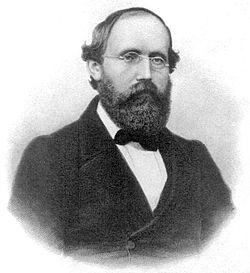
\includegraphics[scale=0.4]{Riemann}
\end{center}

\begin{preuve} Montrons le premier point.

%\begin{itemize}
%\item La fonction $t \mapsto \dfrac{1}{t^{\alpha}}$ est continue sur $[1, +  \infty[$.
%\item L'intégrale est impropre en $+ \infty$.
%\item On distingue deux cas :
%\begin{enumerate}
%\item[$\star$] Si $\alpha=1$, on a pour tout réel $x \geq 1$,
%$$ \int_{1}^x \dfrac{\dt}{t} = \ln(x) \underset{x \rightarrow + \infty}{\rightarrow} + \infty$$
%et ainsi, l'intégrale diverge.
%\item[$\star$] Si $\alpha \neq 1$, on a pour tout réel $x \geq 1$,
%$$ \int_{1}^x \dfrac{\dt}{t^{\alpha}} = \left[ \frac{1}{(1- \alpha) t^{\alpha -1}} \right]_1^x =  \frac{1}{(1- \alpha) x^{\alpha -1}} + \frac{1}{\alpha-1} $$
%Si $\alpha>1$, on a :
%$$ \lim_{x \rightarrow + \infty} \frac{1}{(1- \alpha) x^{\alpha -1}} + \frac{1}{\alpha-1} = \frac{1}{\alpha-1}$$
%et ainsi, l'intégrale converge (et l'on connait la valeur).
%
%\noindent Si $\alpha<1$, on a :
%$$ \lim_{x \rightarrow + \infty} \frac{1}{(1- \alpha) x^{\alpha -1}} + \frac{1}{\alpha-1} = + \infty$$
%et ainsi, l'intégrale diverge.
%\end{enumerate}
%\end{itemize}
%Finalement, on a bien montré que l'intégrale converge si et seulement si $\alpha>1$.

\vspace{10cm}
\end{preuve}

\begin{exa} Montrer le deuxième point de la proposition précédente.
\end{exa}

\begin{prop} L'intégrale $\int_{0}^1 \ln(t) \dt$ converge.
\end{prop}

\begin{prop}
Soit $\lam \in \mathbb{R}$. L'intégrale $\dis \int_0^\pinf e^{-\lam t} \dt$ converge si et seulement si $\lam > 0$.
\end{prop}

\begin{preuve} 
%\begin{itemize}
%\item La fonction $t \mapsto e^{- \lambda t}$ est continue sur $[0, +  \infty[$.
%\item L'intégrale est impropre en $+ \infty$.
%\item On distingue deux cas :
%\begin{enumerate}
%\item[$\star$] Si $\lambda=0$, on a pour tout réel $x \geq 0$,
%$$ \int_{0}^x 1 \dt = x \underset{x \rightarrow + \infty}{\rightarrow} + \infty$$
%\item[$\star$] Si $\lambda \neq 0$, on a pour tout réel $x \geq 0$,
%$$ \int_{0}^xe^{-\lam t} \dt = \left[- \frac{e^{-\lam t}}{\lambda} \right]_{0}^x = - \frac{e^{-\lam x}}{\lambda} + \frac{1}{\lambda}$$
%Si $\lambda>0$, on a alors :
%$$ \lim_{x \rightarrow + \infty}  - \frac{e^{-\lam x}}{\lambda} + \frac{1}{\lambda} = \frac{1}{\lambda}$$
%et ainsi, l'intégrale converge.
%Si $\lambda<0$, on a alors :
%$$ \lim_{x \rightarrow + \infty}  - \frac{e^{-\lam x}}{\lambda} + \frac{1}{\lambda} = + \infty$$
%et ainsi, l'intégrale diverge.
%\end{enumerate}
%Finalement, on a bien montré que l'intégrale converge si et seulement si $\lam>0$.
%\end{itemize}

\vspace{10cm}
\end{preuve}

\subsection{Lien avec l'intégrale \og usuelle \fg}

\begin{prop} Soient $a$, $b$ deux réels tels que $a < b$ et $f$ une fonction continue par morceaux sur $[a,b]$ à valeurs réelles ou complexes. Alors les intégrales de $f$ sur $]a,b]$, $[a,b[$ et $]a,b[$ sont convergentes et leurs valeurs est la valeur de l'intégrale usuelle de $f$ sur $[a,b]$.
\end{prop}

\begin{preuve} Montrons le résultat dans le premier cas. La fonction $f$ est continue par morceaux sur $]a,b]$ donc elle est bornée sur $[a,b]$. On a pour tout $x \in ]a,b]$,

%\begin{align*}
%\left\vert \int_{x}^b f(t) \dt - \int_{a}^b f(t) \dt \right\vert & = \left\vert \int_{a}^x f(t) \dt \right\vert \\
%& \leq (x-a) \sup_{t \in [a,b]} \vert f(t) \vert \\
%\end{align*}
%et on a :
%$$ \lim_{x \rightarrow a^{+}}  (x-a) \sup_{t \in [a,b]} \vert f(t) \vert = 0$$
%ce qui donne le résultat avec le théorème d'encadrement.

\vspace{6cm}
\end{preuve}


\begin{prop} Soient $a$ un réel et $f : ]a,b] \rightarrow \mathbb{K}$ une fonction continue par morceaux. Si la fonction $f$ admet une limite dans $\mathbb{K}$ en $a^{+}$ alors $\int_{a}^b f(t) \dt$ est convergente.


\medskip

\noindent On dit que l'intégrale est \textit{faussement impropre} en $a$ (ou qu'il y a un \textit{faux problème} en $a$).
\end{prop}

\newpage

\begin{preuve} La fonction $f$ est prolongeable par continuité en $a^+$ en une fonction $\tilde{f}$ continue par morceaux sur $[a,b]$. Pour tout $x \in ]a,b]$, on a alors :
$$ \int_{x}^b f(t) \dt = \int_{x}^b \tilde{f}(t) \dt \underset{t \rightarrow a^+}{\longrightarrow} \int_{a}^b \tilde{f}(t) \dt$$
d'après la proposition précédente. Ainsi, l'intégrale est convergente.
\end{preuve}

\medskip

\begin{ex} Étudions la convergence de $I = \int_{0}^1 t \ln(t) \dt$.

\medskip

%\noindent La fonction $t \mapsto t \ln(t)$ est continue sur $]0,1]$ et est prolongeable par continuité en $0$ car :
%$$ \lim_{t \rightarrow 0} t \ln(t) = 0 $$
%d'après le théorème des croissances comparées. Ainsi l'intégrale $I$ est faussement impropre en $0$ donc convergente.

\vspace{3cm}
\end{ex}

\begin{exa} Étudier la convergence de $I = \dis \int_{0}^{1} \dfrac{\sin(t)}{t} \dt$.
\end{exa}

\begin{att} Un faux problème ne peut avoir un sens qu'en une extrémité de $I$ \textit{fini} : un prolongement par continuité en $ \pm \infty$ n'a aucun sens.
\end{att}


\subsection{Quelques propriétés}
\noindent Dans la suite, $a$ et $b$ sont deux éléments de $\overline{\mathbb{R}}$ dans \og le bon ordre \fg .

\begin{prop}[Linéarité de l'intégration] 
Soient $f,g$ deux fonctions continues par morceaux sur $]a,b]$ à valeurs dans $\mathbb{K}$ et $\lambda \in \mathbb{K}$. Si $\int_{a}^b f(t) \dt$ et $\int_{a}^b g(t) \dt$ convergent alors $\int_{a}^b \lambda f(t) + g(t) \dt$ converge et on a :
$$ \int_{a}^b \lambda f(t) + g(t) \dt = \lambda \int_{a}^b f(t) \dt + \int_{a}^b g(t) \dt$$
\end{prop}

\begin{prop}[Positivité, croissance]
Soient $f,g$ deux fonctions continues par morceaux sur $]a,b]$ (avec $a<b$) à valeurs dans $\mathbb{R}$.

\begin{itemize}
\item Si $f$ est positive sur $]a,b]$ et que $\int_{a}^b f(t) \dt$ converge alors $\int_{a}^b f(t) \dt \geq 0$.
\item Si $f \leq g$ sur $]a,b]$ et que $\int_{a}^b f(t) \dt$ et $\int_{a}^b g(t) \dt$ convergent alors $\int_{a}^b f(t) \dt \leq \int_{a}^b g(t) \dt$.
\end{itemize}
\end{prop}

\begin{prop} Soient $f$ une fonctions continue par morceaux sur $]a,b]$ à valeurs dans $\mathbb{C}$. Les assertions suivantes sont équivalentes :

\begin{enumerate}
\item $\int_{a}^b f(t) \dt$ converge.
\item $\int_{a}^b \Re e(f(t)) \dt$ et $\int_{a}^b \Im m(f(t)) \dt$ convergent.
\end{enumerate}
Si ces conditions sont vérifiées, on a alors :
$$ \int_{a}^b f(t) \dt = \int_{a}^b \Re e(f(t)) \dt + i \int_{a}^b \Im m(f(t)) \dt$$
\end{prop}


\begin{rems}
\item On adapte les trois résultats précédents pour les intervalles du type $[a,b[$ et $]a,b[$.
\item Pour prouver les trois résultats précédents, il suffit d'écrire le résultat analogue sur $[x,b]$ (dans le cas \og usuel \fg) puis d'obtenir le résultat par passage à la limite quand $x$ tend vers $a^{+}$.
\end{rems}

\section{Méthodes de calcul d'intégrales généralisées}

\subsection{Utilisation d'une primitive}
\noindent Si $f$ est une fonction continue sur $]a,b]$ et à valeurs dans $\mathbb{K}$ et si $F$ est une primitive de $f$ sur $]a,b]$ alors pour tout $x \in ]a,b]$,
$$ \int_{x}^b f(t) \dt = F(b)-F(x)$$
Donc l'intégrale $\int_{a}^b f(t) \dt$ converge si et seulement si $F$ admet une limite dans $\mathbb{K}$ en $a^{+}$.

\medskip

\noindent On adapte évidemment cette méthode sur les intervalles du type $[a,b[$ et $]a,b[$.
\subsection{Intégration par parties}

\noindent Il faut se méfier de la formule d'intégration par parties dans le cas des intégrales généralisées : une intégrale convergente peut s'écrire comme somme de deux termes qui divergent.

\begin{thm} Soient $f,g$ deux fonctions de classe $\mathcal{C}^1$ sur $]a,b]$. Si la fonction $fg$ a une limite dans $\mathbb{K}$ en $a^+$ alors les intégrales 
$$ \int_{a}^{b} f'(t) g(t) \dt \quad \hbox{ et } \quad \int_{a}^{b} f(t) g'(t) \dt $$
sont de même nature. En notant :
$$ [f(t) g(t)]_{a}^{b} = f(b)g(b) - \lim_{t \rightarrow a^+} f(t)g(t)$$
On a alors en cas de convergence :
$$  \int_{a}^{b} f'(t) g(t) \dt = [f(t) g(t)]_{a}^{b} - \int_{a}^b f(t) g'(t) \dt$$
\end{thm}

\begin{rem} Le résultat s'adapte très facilement sur les intervalles du type $[a,b[$ et $]a,b[$ (dans ce cas, le crochet est constitué de deux limites).
\end{rem}

\begin{preuve} Pour tout $x \in ]a,b]$, on a par intégration par parties \og usuelle \fg :
$$ \int_{x}^{b} f'(t) g(t) \dt = f(b)g(b)-f(x)g(x) - \int_{x}^b f(t) g'(t) \dt$$
La fonction $x \mapsto f(b)g(b)-f(x)g(x)$ admet une limite en $a^+$ ce qui donne le résultat.
\end{preuve}

\medskip

\begin{rem} On peut procéder de deux manières pour utiliser la formule d'intégration par parties :

\begin{itemize}
\item Utiliser le théorème précédent : dans ce cas, il faut très précis sur la rédaction et sur les hypothèses.
\item Utiliser la formule d'intégration par parties usuelle sur un intervalle $[x,b]$ ou $[a,x]$ puis utiliser un passage à la limite.
\end{itemize}
\end{rem}

\medskip


\begin{ex} Montrons que $\dis \int_{0}^1  \dfrac{\ln(t)}{(1+t)^2} \dt$ converge.

%\begin{itemize}
%\item La fonction $t \mapsto \dfrac{\ln(t)}{(1+t)^2}$ est continue sur $]0,1]$. L'intégrale est donc impropre en $0$.
%\item Posons pour tout $t \in ]0,1]$,
%$$ u(t) = \frac{-1}{1+t} \quad \hbox{ et } v(t) = \ln(t)$$
%Alors $u$ et $v$ sont $\mathcal{C}^1$ sur $]0,1]$ et on a pour tout $t \in ]0,1]$,
%$$ u'(t) = \frac{1}{(1+t)^2} \quad \hbox{ et } v'(t) = \frac{1}{t}$$
%Pour tout $x \in ]0,1]$, on a par intégration par parties :
%
%\begin{align*}
%\int_{x}^1  \dfrac{\ln(t)}{(1+t)^2} \dt & = \left[ \frac{-\ln(t)}{1+t} \right]_{x}^1 + \int_{x}^1 \frac{1}{t(t+1)} \dt \\
%& =  \left[ \frac{-\ln(t)}{1+t} \right]_{x}^1 + \int_{x}^1 \frac{1+t-t}{t(t+1)} \dt \\
%&=  \left[ \frac{-\ln(t)}{1+t} \right]_{x}^1 + \int_{x}^1 \frac{1}{t} - \frac{1}{t+1} \dt \\
%& = \left[ \frac{-\ln(t)}{1+t} + \ln(t) - \ln(t+1) \right]_{x}^1 \\
%& = \dfrac{\ln(x)}{1+x}  - \ln(x)+ \ln(x+1) - \ln(2) \\
%& = \ln(x) \left( \frac{1}{1+x} - 1\right) + \ln(x+1)- \ln(2) \\
%& = \frac{-x\ln(x)}{1+x} + \ln(x+1)- \ln(2) \\
%\end{align*}
%et par théorème des croissances comparées, on a :
%$$ \lim_{x \rightarrow 0^+}  \frac{-x\ln(x)}{1+x} + \ln(x+1)- \ln(2) = - \ln(2)$$
%\end{itemize}
%Ainsi, l'intégrale converge et l'on a :
%$$ \int_{0}^1  \dfrac{\ln(t)}{(1+t)^2} \dt = - \ln(2)$$

\vspace{8cm}
\end{ex}

\newpage

$\phantom{test}$

\vspace{4cm}

\begin{exa} Déterminer, pour tout $\lambda>0$, la valeur de :
$$ I(\lambda) = \int_{0}^{+ \infty} \lambda t e^{-\lambda t} \dt$$
\end{exa}

\subsection{Changement de variable}

\begin{thm} Soient $\varphi : ]\alpha, \beta[ \rightarrow ]a,b[= \varphi(]\alpha,\beta[)$ une bijection strictement monotone de classe $\mathcal{C}^1$ et $f : [a,b] \rightarrow \mathbb{K}$ une fonction continue par morceaux. Alors les intégrales :
$$  \int_{\alpha}^{\beta} (f \circ \varphi)(u) \varphi'(u) du \quad \hbox{ et } \quad \int_{a}^b f(t) \dt$$
sont de même nature et en cas de convergence, on a :
$$ \int_{a}^b f(t) \dt= \int_{\alpha}^{\beta} (f \circ \varphi)(u) \vert \varphi'(u) \vert du$$
\end{thm}

\begin{rem} Le terme $\vert \varphi'(u) \vert$ permet de compenser l'inversion des bornes quand $\varphi$ est décroissante.
\end{rem}

\medskip

\begin{preuve} Prouvons le résultat quand $\varphi$ est strictement croissante. Soient $(x,y) \in ]a,b[^2$ et $(w,z) \in ]\alpha, \beta[^2$. 

En utilisant la forme de changement de variable \og usuelle \fg, on a :
$$ \int_{\varphi(w)}^{\varphi(t)} f(t) \dt = \int_{w}^{z} f (\varphi(u)) \varphi'(u) du \quad \hbox{ et } \int_{x}^{y} f(t) \dt = \int_{\varphi^{-1}(x)}^{\varphi^{-1}(y)} f (\varphi(u)) \varphi'(u) du$$
La fonction $\varphi$ est strictement croissante donc :
$$ \varphi(w) \underset{w \rightarrow \alpha^+}{\rightarrow} a^+, \; \varphi(z) \underset{z \rightarrow \beta^-}{\rightarrow} b^-, \; \varphi^{-1}(x) \underset{x \rightarrow a^+}{\rightarrow} \alpha^+, \; \varphi^{-1}(y) \underset{y \rightarrow b^-}{\rightarrow} \beta^-$$
Ainsi les deux intégrales sont simultanément convergentes et sont égales en cas de convergence.

%\vspace{6cm}
\end{preuve} 

%\begin{thm} Soit $\varphi : ]\alpha, \beta[ \rightarrow ]a,b[$ une bijection strictement décroissante de classe $\mathcal{C}$ et $f : [a,b] \rightarrow \mathbb{K}$ une fonction continue par morceaux. Alors les intégrales :
%$$ \int_{\alpha}^{\beta} (f \circ \varphi)(u) \varphi'(u) du \quad \hbox{ et } \int_{a}^b f(t) \dt$$
%sont de même nature et en cas de convergence, on a : 
%$$ \int_{\alpha}^{\beta} (f \circ \varphi)(u) \varphi'(u) du =-  \int_{a}^b f(t) \dt$$
%\end{thm}
%
%\begin{preuve} Similaire à la précédente mais les bornes sont échangées par décroissance de $\varphi$.
%\end{preuve} 

\medskip

\begin{ex} Calculons l'intégrale $I=\dis \int_{0}^1 \frac{1+t^2}{1+t^4} \dt$ à l'aide du changement de variable $t=e^{-u}$.

\vspace{7cm}
%\medskip
%
%\begin{itemize}
%\item La fonction $t \mapsto \frac{1+t^2}{1+t^4}$ est continue sur $[0,1]$ (son intégrale est donc convergente sur $[0,1]$ et celle-ci coïncide avec l'intégrale sur $]0,1]$).
%\item La fonction $t \mapsto e^{-t}$ est une bijection strictement décroissante de classe $\mathcal{C}^1$ de $\mathbb{R}_+$ vers $]0,1]$. Ainsi, d'après le théorème de changement de variable assure $I$ est de même nature (c'est-à-dire convergente) que l'intégrale suivante :
%$$ J = \int_{0}^{+\infty} \frac{1+e^{-2t}}{1+e^{-4t}} (-e^{-t}) \dt =- \int_{0}^{+\infty} \frac{e^t+e^{-t}}{e^{2t}+e^{-2t}} = -\int_{0}^{+\infty} \frac{\ch(t)}{\ch(2t)} \dt $$
%Or, pour tout $t \in \mathbb{R}_+$, $\ch(2t) = \ch(t)^2+ \sh(t)^2 = 1 + 2 \sh(t)^2$ et on a donc :
%\begin{align*}
%\frac{\ch(t)}{\ch(2t)} & = \frac{\ch(t)}{1 + 2 \sh(t)^2} \\
%& = \frac{1}{\sqrt{2}} \frac{\sqrt{2}\ch(t)}{1 + (\sqrt{2} \sh(t))^2} \\
%\end{align*}
%On reconnait la formule $\dfrac{U'}{1+U^2}$ donc :
%$$ J = -\left[ \frac{1}{\sqrt{2}} \arctan (\sqrt{2} t) \right]_{0}^{+\infty} =- \frac{\pi}{2\sqrt{2}}$$
%Or le changement de variable était strictement décroissant donc $I=-J = \dfrac{\pi}{2\sqrt{2}} \cdot$
%\end{itemize}
\end{ex}

\newpage

$\phantom{test}$

\vspace{2cm}
%\section{Critères de comparaison d'intégrales de fonctions positives}
%
%\begin{thm} Soient $f : [a,b[ \rightarrow \mathbb{K}$ et $g : [a,b[ \rightarrow \mathbb{K}$ deux fonctions \textit{positives} et continues par morceaux sur $I$. 
%
%\begin{itemize}
%\item Supposons l'existence d'un réel $c \in [a,b[$ tel que pour tout $t \in [c,b[$, $f(t) \leq g(t)$. Alors :
%
%\begin{enumerate}
%\item La convergence de $\int_{a}^b g(t) \dt$ implique la convergence de  $\int_{a}^b f(t) \dt$. 
%\item La divergence de $\int_{a}^b f(t) \dt$ implique la divergence de  $\int_{a}^b g(t) \dt$. 
%\end{enumerate}
%\item Si $f(t) \underset{ t \rightarrow b^{-}}{=} O(g(t))$ alors la convergence de $\int_{a}^b g(t) \dt$ implique la convergence de  $\int_{a}^b f(t) \dt$. 
%\item Si $f(t) \underset{ t \rightarrow b^{-}}{=} o(g(t))$ alors la convergence de $\int_{a}^b g(t) \dt$ implique la convergence de  $\int_{a}^b f(t) \dt$. 
%\item Si $f(t) \underset{ t \rightarrow b^{-}}{\sim}g(t)$ alors $\int_{a}^b f(t) \dt$ et $\int_{a}^b g(t) \dt$ sont de même nature.
%\end{itemize}
%\end{thm}
%
%\begin{preuve} A taper en modifiant preuves pour intégrabilité !!
%\end{preuve}
%
%\begin{ex} Déterminons la nature de $\dis I= \int_{0}^{+ \infty} \frac{e^{-t}}{\sqrt{t+1}} \dt$.
%
%\medskip
%
%\begin{itemize}
%\item La fonction $t \mapsto \dfrac{e^{-t}}{\sqrt{t+1}}$ est continue sur $[0, + \infty[$. 
%\item L'intégrale est impropre en $+ \infty$.
%\item Pour tout $t \in \mathbb{R}_+$,
%$$ 0 \leq \frac{e^{-t}}{\sqrt{t+1}} \leq e^{-t} $$
%Or l'intégrale $\int_{0}^{+ \infty} e^{-t} \dt$ converge (intégrale de référence) donc par comparaison de fonctions positives, $I$ converge.
%\end{itemize}
%\end{ex}
%
%\begin{ex} Déterminons la nature de $\dis I= \int_{1}^{+ \infty} t+2 - \sqrt{t^2+4t+1} \dt$.
%
%\medskip
%
%
%\begin{itemize}
%\item La fonction $t \mapsto t+2 - \sqrt{t^2+4t+1} $ est continue sur $[1, + \infty[$. 
%\item L'intégrale est impropre en $+ \infty$.
%\item Si $t \rightarrow + \infty$, on a :
%$$ t+2 - \sqrt{t^2+4t+1}  = t+2 - t \sqrt{1 + \frac{4}{t} + \frac{1}{t^2}}$$
%Or si $t \rightarrow + \infty$, $\dis \frac{4}{t} + \frac{1}{t^2} \rightarrow 0$ donc :
%\begin{align*}
%t+2 - \sqrt{t^2+4t+1}  & = t+2 - t  \left( 1 + \frac{1}{2} \left(\frac{4}{t} + \frac{1}{t^2} \right) - \frac{1}{8} \left(\frac{4}{t} + \frac{1}{t^2} \right) + o \left( \frac{1}{t}^2 \right) \right) \\
%& = t+2 - t  \left( 1 + \frac{2}{t} + \frac{1}{2t^2} - \frac{2}{t^2} + o \left( \frac{1}{t^2} \right) \right) \\
%& =  \frac{3}{2t} + o \left( \frac{1}{t} \right) \\
%\end{align*}
%Ainsi :
%$$ t+2 - \sqrt{t^2+4t+1} \underset{ + \infty}{\sim} \frac{3}{2t} $$
%Les fonctions sont continues et positives sur $[1, + \infty[$ (petite inéquation simple pour la première) et l'intégrale $\dis \int_{1}^{+ \infty} \frac{3}{2t} \dt$ diverge (intégrale de Riemann) donc par comparaison de fonctions positives, $I$ diverge.
%\end{itemize}
%\end{ex}

\section{Absolue convergence et intégrabilité}

\subsection{Absolue convergence}

\noindent Dans la suite, $I$ est un intervalle de $\mathbb{R}$ d'extrémités $a$ et $b$ (éléments de $\overline{\mathbb{R}}$).

\begin{defin} Soit $f : I \rightarrow \mathbb{K}$ une fonction continue par morceaux. On dit que que l'intégrale $\int_{a}^b f(x) \dx$ est \textit{absolument convergente} si $\int_{a}^b \vert f(x) \vert \dx$ est convergente.
\end{defin}

\begin{prop} Soit $f : I \rightarrow \mathbb{K}$ une fonction continue par morceaux. Si l'intégrale $\int_{a}^b f(x) \dx$ est absolument convergente alors elle est convergente et on a :
$$ \left\vert \int_{a}^b  f(x)  \dx \right\vert \leq \int_{a}^b \vert f(x) \vert \dx $$
\end{prop}

\begin{preuve} Faisons la preuve dans le cas où $I = ]a,b]$. 

%Posons $h = \Re e(f)$, $h^+ = \max \lbrace 0,h \rbrace$ et $h^{-}= \max \lbrace 0, -h \rbrace$. On a $h=h^+ - h^{-}$ et $\vert h = \vert h^+ + h^{-}$ et ainsi :
%$$ h^+ = \frac{1}{2} ( \vert h \vert + h) \quad \hbox{ et } \frac{1}{2} ( \vert h \vert -h ) $$
%Les fonctions $h^+$ et $h^{-}$ sont ainsi continues par morceaux sur $I$ et on a :
%$$ 0 \leq h^+ \leq \vert h \vert  = \vert \Re (f) \vert \leq \sqrt{Re (f)^2 + \Im m(f)^2} = \vert f \vert $$
%et de même :
%$$ 0 \leq h^{-} \leq \vert h \vert \leq \vert f \vert $$
%Pour tout $x \in ]a,b]$ et par croissance de l'intégrale, on a :
%$$ \int_{x}^b h^+(t) \dt \leq \int_{x}^b \vert f(t) \vert \dt $$
%Or la fonction $t \mapsto \vert f(t) \vert$ est positive et sont intégrale sur $]a,b]$ est convergente par hypothèse donc la fonction :
%$$ x \mapsto \int_{x}^b \vert f(t) \vert \dt$$
%est majorée sur $I$. Ainsi la fonction :
%$$ x \mapsto \int_{x}^b h^+(t) \dt$$ 
%est aussi majorée sur $I$ et comme $t \mapsto h^+ (t) $ est positive, on en déduite que $\int_{a}^b h^+(t) \dt$ converge. De même, on montre que   $\int_{a}^b h^{-}(t) \dt$ converge. Sachant que $h=h^+-h^{-}$, on en déduit que $\int_{a}^b h(t) \dt$. On procède de la même manière pour la partie imaginaire de $f$ ce qui implique que  $\int_{a}^b f(t) \dt$ converge.
%
%\medskip
%
%\noindent Pour obtenir l'inégalité, il suffit d'utiliser l'inégalité triangulaire \og usuelle \fg sur les segments $[x,b]$ puis de passer à la limite quand $x$ tend vers $a^+$.


\vspace{11cm}
\end{preuve}

\begin{defin} Soit $f : I \rightarrow \mathbb{K}$ une fonction continue par morceaux. On dit que que $f$ est \textit{intégrable} sur $I$ si l'intégrale $\int_{a}^b f(x) \dx$ est absolument convergente. Dans ce cas, cette intégrale converge et on pourra noter la valeur de cette intégrale par l'une des notations suivantes :
$$ \int_{a}^b f(x) \dx, \quad \int_{I} f(x) \dx, \quad \int_I f$$
\end{defin}

\begin{rems}
\item Si une fonction est intégrable sur $I$ alors $\int_{a}^b f(x) \dx$ converge. La réciproque est \textit{fausse} : il existe des fonctions dont l'intégrale converge mais que ne sont pas intégrables sur l'intervalle considéré : voir TD.
\item Si une fonction continue par morceaux sur $I$ est à valeurs réelles et de signe \textit{constant} alors :
$$ f \hbox{ est intégrable sur I} \Longleftrightarrow \int_{a}^b f(x) \dx \hbox{ converge}$$
\item Si une fonction $f$ définie sur $I$ est à valeurs complexes, alors :
$$ \int_{a}^b f(x) \dx \hbox{ converge absolument } \Longleftrightarrow \int_{a}^b \Re e(f)(x) \dx \hbox{ et }  \int_{a}^b \Im m(f)(x) \dx \hbox{ convergent absolument} $$
\end{rems}

\begin{prop} Si une fonction $f$ est intégrable sur un intervalle $I$, elle l'est sur tout sous-intervalle de $I$.
\end{prop}

\begin{prop} Si $f$ est continue par morceaux sur $I=[a,b]$ ($a$, $b$ deux réels tels que $a <b$)  alors $f$ est intégrable sur $[a,b]$.
\end{prop}

\begin{preuve}
La fonction $\vert f \vert$ est continue par morceaux sur $[a,b]$ donc l'intégrale existe (au sens usuel) donc converge.
\end{preuve}


\subsection{Critères de comparaison}

\begin{thm} Soient $f : [a,b[ \rightarrow \mathbb{K}$ et $g : [a,b[ \rightarrow \mathbb{K}$ deux fonctions continues par morceaux.

\begin{itemize}
\item Si $\vert f \vert \leq \vert g \vert$ sur $[a,b[$ et si $g$ est intégrable sur $[a,b[$ alors $f$ est intégrable sur $[a,b[$.
\item Si $f(t) \underset{ t \rightarrow b^{-}}{=} O(g(t))  $ et si $g$ est intégrable sur $[a,b[$ alors $f$ est intégrable sur $[a,b[$.
\item Si $f(t) \underset{ t \rightarrow b^{-}}{=} o(g(t))  $ et si $g$ est intégrable sur $[a,b[$ alors $f$ est intégrable sur $[a,b[$.
\item Si $f(t) \underset{ t \rightarrow b^{-}}{\sim}g(t)$ alors $f$ est intégrable sur $[a,b[$ si et seulement si $g$ est intégrable sur $[a,b[$.
\end{itemize}
\end{thm}

\begin{rem} On adapte les énoncés dans le cas d'un intervalle de la forme $]a,b]$.
\end{rem}

\begin{preuve}
%
%\begin{itemize}
%\item Pour tout $x \in [a,b[$ et par croissance de l'intégrale, on a :
%$$ \int_{a}^x \vert f(t) \vert \dt \leq \int_{a}^x \vert g(t) \vert \dt$$
%Or la fonction $t \mapsto \vert g(t) \vert$ est positive et $g$ est intégrable sur $[a,b[$ donc la fonction
%$$ x \mapsto \int_{a}^x \vert g(t) \vert \dt$$
%est majorée sur $[a,b[$. Ainsi, la fonction 
%$$  x \mapsto \int_{a}^x \vert f(t) \vert \dt$$
%est majorée sur $[a,b[$ et la fonction $t \mapsto \vert f(t) \vert$ est positive sur $[a,b[$ donc $f$ est intégrable sur $[a,b[$.
%\item Supposons que $f(t) \underset{ t \rightarrow b^{-}}{=} O(g(t))$. Il existe alors un réel $K>0$ et $c \in [a,b[$ tel que pour tout $t \in [c,b[$, 
%$$ \vert f(t) \vert \leq K \vert g(t) \vert $$
%La fonction $g$ est intégrable sur $[a,b[$ donc elle est intégrable sur $[a,c[$ (JUSTIFIER AVANT) donc d'après le cas précédent, la fonction $f$ est intégrable sur $[c,b[$. De plus, $f$ est continue sur $[a,c]$ donc elle est intégrable sur cette intervalle (JUSTIFIER AVANT) donc par la relation de Chasles, $f$ est intégrable sur $[a,b[$.
%\item Si $f(t) \underset{ t \rightarrow b^{-}}{=} o(g(t))$ alors $f(t) \underset{ t \rightarrow b^{-}}{=} O(g(t))$ et on sa ramène au cas précédent.
%\item Si $f(t) \underset{ t \rightarrow b^{-}}{\sim}g(t)$ alors $f(t) \underset{ t \rightarrow b^{-}}{=} O(g(t))$ et $g(t) \underset{ t \rightarrow b^{-}}{=} (f(t))$ donc on sa ramène au deuxième cas.
%\end{itemize}

\vspace{10cm}
\newpage

%$\phantom{test}$
%
%\vspace{5cm}
\end{preuve}

\begin{ex} Montrons que $x \mapsto \dfrac{\cos(x)}{x^2}$ est intégrable sur $[1,+ \infty[$.

\vspace{4cm}
\end{ex}

\begin{exa} Montrer que $\dis x \mapsto \dfrac{1}{x} \sin \left( \frac{1}{x} \right)$ est intégrable sur $[1,+ \infty[$.
\end{exa} 

\medskip

\noindent \textbf{Remarque importante dans la pratique :} Si la fonction $f$ est positive sur $[a,b[$, alors $f$ est intégrable si et seulement si son intégrale sur $[a,b[$ converge ce qui donne le critère de comparaison suivant :

\medskip

\begin{thm}[Critère de comparaison] Soient $f$ et $g$ deux fonctions continues par morceaux sur $[a,b[$ à \textit{valeurs positives}.

\begin{itemize}
\item Si pour tout $t \in [a,b[$, $f(t) \leq g(t)$ alors :

\begin{enumerate}
\item Si $ \int_{a}^{b} g(t) \dt$ converge alors $ \int_{a}^{b} f(t) \dt$ converge.
\item Si $ \int_{a}^{b} f(t) \dt$ diverge alors $ \int_{a}^{b} g(t) \dt$ diverge.
\end{enumerate}
\item Si $f(t) \underset{ t \rightarrow b^{-}}{=} O(g(t))$ et si $ \int_{a}^{b} g(t) \dt$ converge alors $ \int_{a}^{b} f(t) \dt$ converge.
\item Si $f(t) \underset{ t \rightarrow b^{-}}{=} o(g(t))  $ et si $ \int_{a}^{b} g(t) \dt$ converge alors $ \int_{a}^{b} f(t) \dt$ converge.
\item Si $f(t) \underset{ t \rightarrow b^{-}}{\sim}g(t)$ alors $\int_{a}^{b} f(t) \dt$ et $\int_{a}^{b} g(t) \dt$ sont de même nature.
\end{itemize}
\end{thm}

\begin{rems}
\item Pour la première propriété, il suffit que $f \leq g$ sur un intervalle de la forme $[c,b[$ (sur $[a,c]$ la fonction est continue par morceaux donc son intégrale sur $[a,c]$ converge).
\item Si $f$ est continue par morceaux sur $[a,b[$ et positive alors :
$$ x \mapsto \int_{a}^x f(t) \dt$$
est croissante donc si l'intégrale $\int_{a}^{b} f(t) \dt$ diverge cela signifie que :
$$ \lim_{x \rightarrow b} \int_{a}^x f(t) \dt = + \infty$$
\end{rems}

\subsection{Des exemples}

\noindent \textbf{Exemple 1 : Fraction rationnelle}

\noindent Étudions la nature de $\dis \int_{0}^{+ \infty} \frac{2x}{x^2+x+1} \dx$.

\vspace{5cm}

\begin{exa} Étudier la nature de $\dis \int_{0}^{+ \infty} \frac{x}{x^3+x^2+1} \dx$.
\end{exa}

\medskip

\noindent \textbf{Exemple 2 : Intégrales de Bertrand}

\medskip

\noindent Posons pour tout $(\alpha, \beta) \in \mathbb{R}^2$, 
$$ I(\alpha, \beta) = \int_{2}^{+ \infty} \frac{\dx}{x^{\alpha} \ln(x)^{\beta}}$$

\begin{itemize}
\item La fonction $f: x \mapsto \dis \frac{1}{x^{\alpha} \ln(x)^{\beta}}$ est continue sur $[2, + \infty[$.
\item Si $\alpha>1$, on montre que $\dis f(x)=o \left( \frac{1}{x^{\gamma}} \right)$ où $1 < \gamma < \alpha$ et on montre que l'intégrale converge par critère de comparaison.
\item Si $\alpha<1$, on montre que $xf(x) \geq 1$ à partir d'un certain rang en calculant la limite en $+ \infty$ et on montre que l'intégrale diverge par critère de comparaison.
\item Si $\alpha=1$, l'intégrale $I(1, \beta)$ converge si et seulement si $\beta>1$. On revient pour cela à la définition en calculant \og l'intégrale partielle \fg .
\end{itemize}

\medskip

\noindent Étudions la nature de $I=\dis \int_{1}^{+ \infty} \frac{\ln(t)}{1+t^2} \dt$.

\vspace{5cm}

\noindent Étudions la nature de $J=\dis \int_{0}^{+ \infty} \frac{\ln(t)}{1+t^2} \dt$.

\vspace{5cm}

\noindent Étudions la nature de $K=\dis \int_{1}^{+ \infty} \frac{1}{t \ln(t)^3} \dt$.

\vspace{5cm}

\newpage
\noindent Étudions la nature de $L=\dis \int_{1}^{+ \infty} \frac{\ln(t)}{\sqrt{t}} \dt$.



\vspace{5cm}

\begin{att} La méthode précédente fonctionne quand l'intégrale est impropre en $+ \infty$.
\end{att}

\begin{exa} Donner la nature de $\dis \int_{0}^{+ \infty} \frac{\ln(t)}{t^3+t^2+1} \dt$.
\end{exa}

%\medskip
%
%\noindent \textbf{Exemple 3 : Règle du \og $t^{\alpha}f(t)$ \fg }
%
%\noindent Parfois, étudier la limite de $t^{\alpha}f(t)$ quand $t \rightarrow + \infty$ où $t \rightarrow 0$ avec un bon choix de $\alpha$ permet de montrer que l'intégrale de $f$ converge ou diverge sur l'intervalle considéré.
%
%\medskip
%
%\noindent Étudions la nature de $\dis \int_{0}^{+ \infty} \frac{\cos(t)}{1+t^2} \dt$.
%
%\vspace{5cm}
%
%\noindent Étudions la nature de $\dis \int_{1}^{+ \infty} \frac{1}{\ln(1+t)} \dt$.
%
%\vspace{5cm}
%
%
%\begin{exa} Étudier la nature de $\dis \int_{0}^{+ \infty} P(t) e^{-t^2} \dt$ où $P$ est une fonction polynômiale non nulle.
%\end{exa}

\medskip

\noindent \textbf{Exemple 3 : avec une exponentielle ...}

\noindent Étudions la nature de $\dis \int_{0}^{+ \infty} P(t) e^{-t^2} \dt$ où $P$ est une fonction polynômiale non nulle.

\vspace{6cm}


%\noindent \textbf{Exemple 4 : Intégrales de Riemann translatées}
%
%\noindent Voir TD.

\subsection{Quelques propriétés}

\begin{thm} L'ensemble des fonctions continues par morceaux intégrables sur un intervalle $I$ et à valeurs dans $\mathbb{K}$ est $\mathbb{K}$-espace vectoriel.
\end{thm}

\begin{prop} Soit $f$ une fonction \textit{continue} et intégrable sur un intervalle $I$. Alors :
$$ \int_{I} \vert f(t) \vert \dt=0 \Longrightarrow f \hbox{ est nulle sur } I $$
\end{prop}

\section{Suites et séries de fonctions intégrables}

\newpage

\begin{thm}[convergence dominée]
Soit $(f_n)_{n \geq 0}$ une suite de fonctions continues par morceaux sur $I$ et à valeurs dans $\mathbb{K}$. Supposons que :
\begin{enumerate}
\item La suite $(f_n)_{n \geq 0}$ converge simplement vers une fonction $f$ continue par morceaux sur $I$.
\item Il existe une fonction $\varphi : I \rightarrow \mathbb{K}$, continue par morceaux et intégrable sur $I$, telle que pour tout $n \geq 0$, $\vert f_n \vert \leq \varphi$.
\end{enumerate}
Alors :
\begin{itemize}
\item Pour tout $n \geq 0$, $f_n$ est intégrable sur $I$.
\item $f$ est intégrable sur $I$.
\item $\dis \int_{I} f_n(t) \dt \underset{n \rightarrow + \infty}{ \longrightarrow} \int_{I} f(t) \dt$
\end{itemize}
\end{thm}

\begin{rem} Le fait que chaque fonction $f_n$ soit intégrable provient du fait que $\vert f_n \vert \leq \varphi$ et que $\varphi$ soit intégrable.
\end{rem}

\begin{ex} Déterminons $\dis \lim_{n \rightarrow + \infty} \int_{0}^{+ \infty} \frac{e^{- \frac{x}{n}}}{1+x^2} \dx$.

%\medskip
%
%\noindent Posons pour tout $n \geq 1$, $f_n$ la fonction définie sur $\mathbb{R}_+$ par :
%$$ \forall x \in \mathbb{R}_+, \; f_n(x) = \frac{e^{- \frac{x}{n}}}{1+x^2}$$
%
%\begin{itemize}
%\item Pour tout $n \geq 1$, $f_n$ est continue sur $\mathbb{R}_+$.
%\item Pour tout $x \in \mathbb{R}$,
%$$ -\frac{x}{n} \underset{n \rightarrow + \infty}{\longrightarrow} 0$$
%et donc par continuité de l'exponentielle, on en déduit que :
%$$ f_n(x) \underset{n \rightarrow + \infty}{\longrightarrow} \frac{1}{1+x^2}$$
%Ainsi, $(f_n)_{n \geq 1}$ converge simplement vers $f$ sur $\mathbb{R}_+$ où pour tout $x \in \mathbb{R}_+$,
%$$ f(x) = \frac{1}{1+x^2}$$
%La fonction $f$ est continue sur $\mathbb{R}_+$.
%\item Pour tout $n \geq 1$ et tout $x \in \mathbb{R}_+$, on a :
%$$ \vert f_n(x) \vert \leq \frac{1}{1+x^2} = f(x)$$
%La fonction $f$ est intégrable sur $\mathbb{R}^+$ car pour tout $A>0$,
%$$ \int_{0}^{A} \vert f(x) \vert \dx  = \arctan(A) \underset{n \rightarrow + \infty}{\longrightarrow} \frac{\pi}{2}$$
%\end{itemize}
%Ainsi, par théorème de convergence dominée, on en déduit que pour tout $n \geq 1$, $f_n$ est intégrable sur $\mathbb{R}_+$, et que :
%$$ \lim_{n \rightarrow + \infty} \int_{0}^{+ \infty} f_n(x) \dx = \int_{0}^{+ \infty} f(x) \dx = \frac{\pi}{2}$$

\vspace{11.5cm}
\end{ex}

%\newpage
%
%$\phantom{test}$
%
%\vspace{3cm}

\begin{ex} Déterminons $\dis \lim_{n \rightarrow + \infty} \int_{0}^{\frac{\pi}{4}} \tan(t)^n \dt$.

\medskip


\vspace{10cm}
%\noindent Posons pour tout $n \geq 1$, $f_n$ la fonction définie sur $[0, \frac{\pi}{4}]$ par :
%$$ \forall x \in [0, \frac{\pi}{4}], \; f_n(x) = \tan(x)^n$$
%
%\begin{itemize}
%\item Pour tout $n \geq 1$, $f_n$ est continue sur $[0, \frac{\pi}{4}]$.
%\item Pour tout $x \in [0, \frac{\pi}{4}[$, $\tan(x) \in [0,1[$ donc :
%$$ f_n(x) \underset{n \rightarrow + \infty}{\longrightarrow}0$$
%et si $x= \frac{\pi}{4}$,
%$$ f_n(\frac{\pi}{4})  \underset{n \rightarrow + \infty}{\longrightarrow}1$$
%Ainsi, $(f_n)_{n \geq 1}$ converge simplement vers $f$ sur $[0, \frac{\pi}{4}]$ où pour tout $x \in  [0, \frac{\pi}{4}]$, $f(x)=0$ si $x< \frac{\pi}{4}$ et $f(\frac{\pi}{4})=1$. La fonction $f$ est continue par morceaux sur $[0, \frac{\pi}{4}]$.
%\item Pour tout $n \geq 1$ et tout $x \in [0, \frac{\pi}{4}]$, on a :
%$$ \vert f_n(x) \vert \leq 1$$
%et $x \mapsto 1$ est intégrable sur $[0, \frac{\pi}{4}]$.
%\end{itemize}
%Ainsi, par théorème de convergence dominée, on en déduit que pour tout $n \geq 1$, $f_n$ est intégrable sur $\mathbb{R}_+$, que $f$ aussi (même si c'est clair) et que :
%$$\lim_{n \rightarrow + \infty} \int_{0}^{\frac{\pi}{4}} f_n(x) \dx = \int_{0}^{\frac{\pi}{4}} f(x) \dx = 0$$
\end{ex}

\newpage

$\phantom{test}$

\vspace{4cm}

\begin{rem} Dans l'exemple précédent, il n'y a pas convergence uniforme (limite simple non continue sur $[0, \pi/4]$) donc on ne peut pas appliquer le théorème d'interversion limite-intégrale.
\end{rem}

%\begin{ex} Déterminer $\dis \lim_{n \rightarrow + \infty} \int_{1}^n \dfrac{1}{x} \left(1 - \frac{x}{n} \right)^n \dx$.
%
%Préciser qu'il faut poser $f_n$ selon l'intervalle...
%\end{ex}

\begin{thm}[Intégration terme à terme]
Soit $\dis \Sum{n \geq 0}{} f_n$ une série de fonctions définies sur $I$. Supposons que :
\begin{enumerate}
\item Pour tout entier $n \geq 0$, $f_n$ est continue par morceaux et intégrable sur $I$.
\item $\Sum{n \geq 0}{} f_n$ converge simplement sur $I$ vers une fonction somme $S=\dis \Sum{n=0}{+\infty} f_n$ continue par morceaux sur $I$.
\item La série numérique $ \Sum{n \geq 0}{} \dis \int_{I} \vert f_n(t) \vert \dt$ converge.
\end{enumerate}
Alors :
\begin{itemize}
\item $S$ est intégrable sur $I$.
\item $\dis \int_{I} S(t) \dt =  \Sum{n=0}{+\infty} \dis \int_{I} f_n(t) \dt$.
\end{itemize}
\end{thm}

\begin{ex} Pour tout entier naturel $n \geq 1$, on définit la fonction $f_n : \mathbb{R}_+ \rightarrow \mathbb{R}$ par :
$$ \forall x \in \mathbb{R}_+, \; f_n(x)=xe^{-nx}$$

\noindent Utilisons le théorème d'intégration terme à terme pour obtenir une jolie égalité :
%
%\begin{enumerate}
%\item $f_n$ continue et intégrable sur $\mathbb{R}_+$.
%\item $S(x)= \dfrac{x}{e^{x}-1}$ si $x \neq 0$ et $0$ si $x=0$ donc continue par morceaux sur $\mathbb{R}_+$.
%\item l'intégrale de la valeur absolue de $f_n$ est égal à simplement l'intégrale qui donne $\dfrac{1}{n^2}$ (intégration par parties). Donc la série des intégrales des valeurs absolue converge ...
%\item Conclusion avec l'intégrale de $S$ égale à zeta(2).
%\end{enumerate}

\vspace{10cm}
\end{ex}

\newpage

$\phantom{test}$

\vspace{3cm}
\section{Comparaison série-intégrale}

\begin{thm} Soit $f$ une fonction continue par morceaux sur $[0,+ \infty[$, positive et décroissante. Les assertions suivantes sont équivalentes :

\begin{enumerate}
\item La série $\Sum{n \geq 0}{} f(n)$ converge.
\item $f$ est intégrable sur $[0, + \infty[$
\end{enumerate}
\end{thm}

\begin{rem} Le résultat s'adapte facilement si $f$ est définie sur $[m, + \infty[$ avec $m$ entier.
\end{rem} 

\begin{preuve}

\vspace{13.2cm}
\end{preuve}

\begin{exa} Montrer que $\Sum{n \geq 2}{} \dfrac{1}{n \sqrt{\ln(n)}}$ diverge.
\end{exa}
\end{document}



